% Editable vector schematic. Sources: pinned parent_config.json,
% periodic_config.json and endpoint_selection.json in encoder_chemistry_20260930.
% Different runs have different counters; 1209k is not 19k more parent updates.
\documentclass[tikz,border=0pt]{standalone}
\usepackage{fontspec}
\setsansfont{LiberationSans}[Path=../../shared/assets/,Extension=.ttf,UprightFont=*-Regular,BoldFont=*-Bold]
\usetikzlibrary{arrows.meta,calc}
\definecolor{ink}{HTML}{0C0C0C}
\definecolor{muted}{HTML}{63676B}
\definecolor{copycolor}{HTML}{A36F23}
\definecolor{accent}{HTML}{007C83}
\definecolor{teacherfill}{HTML}{FBF5EA}
\definecolor{comparefill}{HTML}{EDF6F5}
\hyphenpenalty=10000\exhyphenpenalty=10000
\begin{document}
\ifdefined\SlideDiagram
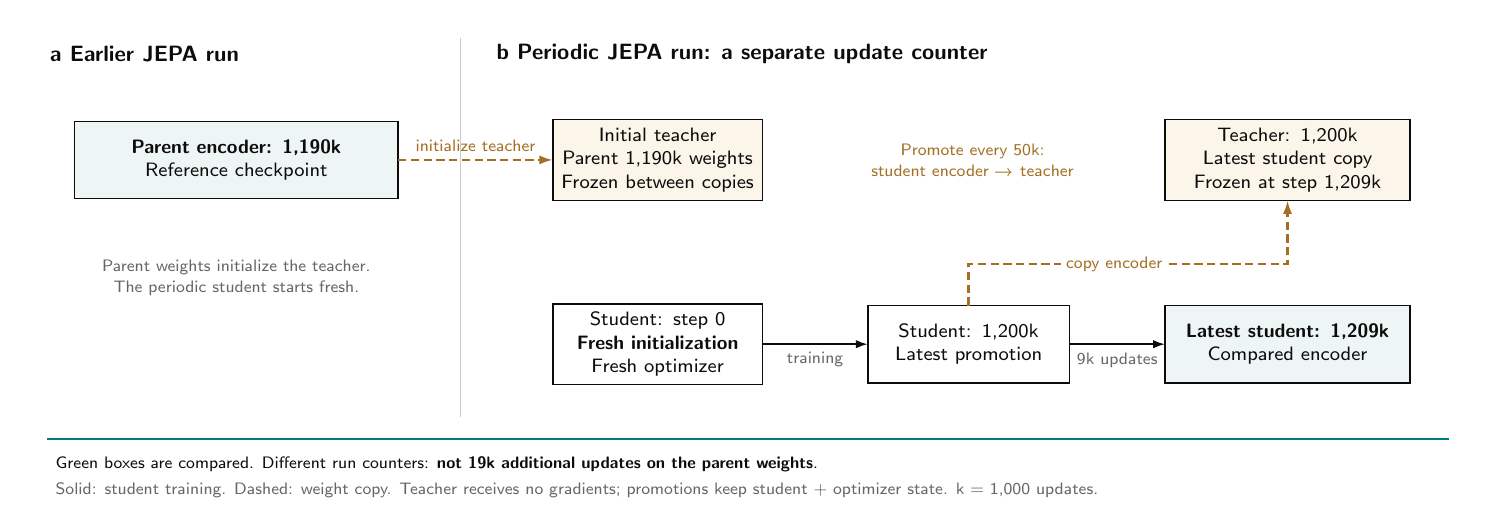
\begin{tikzpicture}[x=1cm,y=1cm,
 every node/.style={font=\sffamily\fontsize{7}{8.5}\selectfont,text=ink,align=center,inner sep=3pt,outer sep=0pt},
 box/.style={draw=ink,line width=.55pt,minimum height=.98cm},
 flow/.style={-{Latex[length=1.5mm,width=1.05mm]},line width=.65pt,draw=ink},
 copy/.style={-{Latex[length=1.7mm,width=1.15mm]},line width=.85pt,draw=copycolor,dash pattern=on 3pt off 1.6pt},
 note/.style={font=\sffamily\fontsize{6.3}{7.6}\selectfont,text=muted},
 panel/.style={anchor=west,font=\sffamily\bfseries\fontsize{8}{10}\selectfont}]
\path[use as bounding box] (0,0) rectangle (18.3,6.05);
\node[panel] at (.18,5.72) {a  Earlier JEPA run};
\node[panel] at (5.85,5.72) {b  Periodic JEPA run: a separate update counter};
\draw[muted!35,line width=.4pt] (5.5,1.1)--(5.5,5.92);
\node[box,text width=3.9cm,fill=comparefill] (sp) at (2.65,4.37)
 {\textbf{Parent encoder: 1,190k}\\Reference checkpoint};
\node[box,text width=2.45cm,fill=teacherfill] (sti) at (8.0,4.37)
 {Initial teacher\\Parent 1,190k weights\\Frozen between copies};
\node[box,text width=2.9cm,fill=teacherfill] (stl) at (16.0,4.37)
 {Teacher: 1,200k\\Latest student copy\\Frozen at step 1,209k};
\draw[copy] (sp.east)--node[above,note,text=copycolor] {initialize teacher}(sti.west);
\node[note,text=copycolor,text width=3.8cm] at (12.0,4.37)
 {Promote every 50k:\\student encoder → teacher};
\node[note,text width=4.7cm] at (2.65,2.87)
 {Parent weights initialize the teacher.\\The periodic student starts fresh.};
\node[box,text width=2.45cm] (ssf) at (8.0,2.03)
 {Student: step 0\\\textbf{Fresh initialization}\\Fresh optimizer};
\node[box,text width=2.35cm] (ssp) at (11.95,2.03)
 {Student: 1,200k\\Latest promotion};
\node[box,text width=2.9cm,fill=comparefill] (ssl) at (16.0,2.03)
 {\textbf{Latest student: 1,209k}\\Compared encoder};
\draw[flow] (ssf.east)--node[below,note] {training}(ssp.west);
\draw[flow] (ssp.east)--node[below,note] {9k updates}(ssl.west);
\draw[copy] (ssp.north)--(11.95,3.05)--(16.0,3.05)--(stl.south);
\node[note,text=copycolor,fill=white,inner sep=2pt] at (13.8,3.05) {copy encoder};
\draw[accent,line width=.8pt] (.25,.83)--(18.05,.83);
\node[anchor=west,font=\sffamily\fontsize{6.5}{8}\selectfont] at (.25,.51)
 {Green boxes are compared. Different run counters: \textbf{not 19k additional updates on the parent weights}.};
\node[anchor=west,note,font=\sffamily\fontsize{6}{7.2}\selectfont] at (.25,.17)
 {Solid: student training. Dashed: weight copy. Teacher receives no gradients; promotions keep student + optimizer state. k = 1,000 updates.};
\end{tikzpicture}
\else
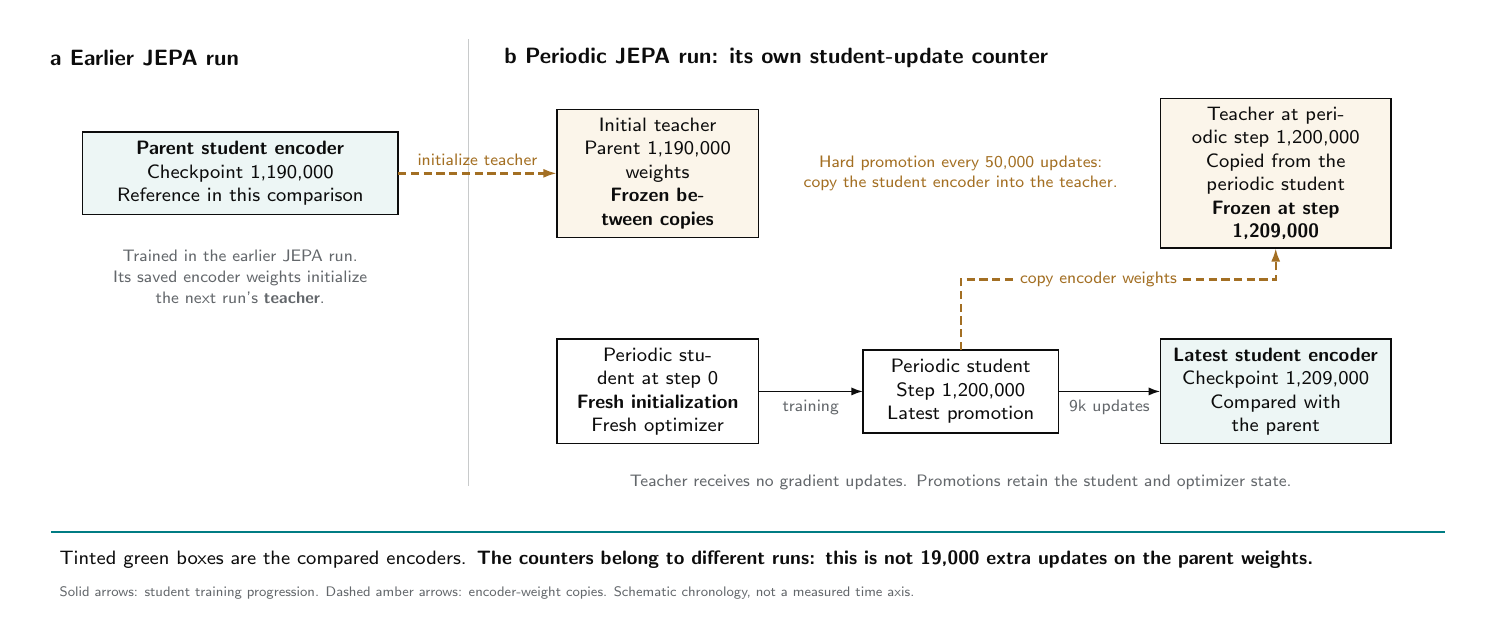
\begin{tikzpicture}[x=1cm,y=1cm,
 every node/.style={font=\sffamily\fontsize{7}{8.5}\selectfont,text=ink,align=center,inner sep=3pt,outer sep=0pt},
 box/.style={draw=ink,line width=.55pt,minimum height=1.05cm},
 flow/.style={-{Latex[length=1.5mm,width=1.05mm]},line width=.65pt,draw=ink},
 copy/.style={-{Latex[length=1.7mm,width=1.15mm]},line width=.85pt,draw=copycolor,dash pattern=on 3pt off 1.6pt},
 note/.style={font=\sffamily\fontsize{6.1}{7.5}\selectfont,text=muted},
 panel/.style={anchor=west,font=\sffamily\bfseries\fontsize{8}{10}\selectfont}]
\path[use as bounding box] (0,0) rectangle (18.3,7.4);
\node[panel] at (.18,7.02) {a  Earlier JEPA run};
\node[panel] at (5.95,7.02) {b  Periodic JEPA run: its own student-update counter};
\draw[muted!35,line width=.4pt] (5.6,1.58)--(5.6,7.25);

\node[box,text width=3.8cm,fill=comparefill] (parent) at (2.7,5.55)
 {\textbf{Parent student encoder}\\Checkpoint 1,190,000\\Reference in this comparison};
\node[note,text width=4.8cm] at (2.7,4.24)
 {Trained in the earlier JEPA run.\\Its saved encoder weights initialize\\the next run's \textbf{teacher}.};
\node[box,text width=2.35cm,fill=teacherfill] (initialteacher) at (8.0,5.55)
 {Initial teacher\\Parent 1,190,000 weights\\\textbf{Frozen between copies}};
\node[box,text width=2.72cm,fill=teacherfill] (lastteacher) at (15.85,5.55)
 {Teacher at periodic step 1,200,000\\Copied from the periodic student\\\textbf{Frozen at step 1,209,000}};
\draw[copy] (parent.east)--node[above,note,text=copycolor] {initialize teacher}(initialteacher.west);
\node[note,text=copycolor,text width=4.7cm] at (11.85,5.55)
 {Hard promotion every 50,000 updates:\\copy the student encoder into the teacher.};

\node[box,text width=2.35cm] (fresh) at (8.0,2.78)
 {Periodic student at step 0\\\textbf{Fresh initialization}\\Fresh optimizer};
\node[box,text width=2.27cm] (promoted) at (11.85,2.78)
 {Periodic student\\Step 1,200,000\\Latest promotion};
\node[box,text width=2.72cm,fill=comparefill] (latest) at (15.85,2.78)
 {\textbf{Latest student encoder}\\Checkpoint 1,209,000\\Compared with the parent};
\draw[flow] (fresh.east)--node[below,note] {training}(promoted.west);
\draw[flow] (promoted.east)--node[below,note] {9k updates}(latest.west);
\draw[copy] (promoted.north)--(11.85,4.2)--(15.85,4.2)--(lastteacher.south);
\node[note,text=copycolor,fill=white,inner sep=2pt] at (13.6,4.2) {copy encoder weights};
\node[note,text width=10.8cm] at (11.85,1.62)
 {Teacher receives no gradient updates. Promotions retain the student and optimizer state.};

\draw[accent,line width=.8pt] (.3,1.0)--(18.0,1.0);
\node[anchor=west,text width=17.5cm,align=left,font=\sffamily\fontsize{6.7}{8.3}\selectfont] at (.3,.65)
 {Tinted green boxes are the compared encoders. \textbf{The counters belong to different runs: this is not 19,000 extra updates on the parent weights.}};
\node[anchor=west,note,font=\sffamily\fontsize{5.5}{6.7}\selectfont] at (.3,.22)
 {Solid arrows: student training progression. Dashed amber arrows: encoder-weight copies. Schematic chronology, not a measured time axis.};
\end{tikzpicture}
\fi
\end{document}
